% Use the following line for draft mode (double spaced, single column)
\documentclass[preprint,pre,floats,aps,amsmath,amssymb]{revtex4}

% Use the following line for journal mode (single spaced, double column)
%\documentclass[twocolumn,pre,floats,aps,amsmath,amssymb]{revtex4}

\usepackage[]{graphicx}
\usepackage{subcaption}
\captionsetup{compatibility=false}
\usepackage{wrapfig} %for wrapping text around images
\usepackage{bm} %bold fonts, e.g. vectors
\usepackage{multirow} %multirow in tables
\usepackage{afterpage} %when you need clearpage, but don't want an empty page
%\renewcommand{\baselinestretch}{1} %for single-spaced

\graphicspath{{pics/}}


\begin{document}

\title{HgCr$_2$Se$_4$ as a Weyl semimetal}
\author{M\'{a}t\'{e} Hartstein}
\email{mate.hartstein@chch.ox.ac.uk}
\affiliation{Christ\:Church, University\:of\:Oxford}
\date{\today}

\clearpage\maketitle
\thispagestyle{empty}

%%%%%%%%%%%%%%%%%%%%%%%%%%%%%%%%%%%%%%%%%%%%%%%%%%%%%%%%%%%
%%%%%%%%%%%%%%%%%%%%%%%%%%%%%%%%%%%%%%%%%%%%%%%%%%%%%%%%%%%

\section{Introduction}
\label{sec:intro}

Topological insulators have become a widely pursued subject in condensed matter physics. A recently proposed related phase is the Weyl semimetal phase (WSM) (Wan et al. (2011) \cite{wan}), which is also gaining popularity, with important experimental results yet to come.
 
This phase is identified by a band structure where two bands accidentally touch at isolated points in the Brillouin zone, which are reminiscent of massless Dirac fermions (or so-called Weyl fermions). This is subject to the condition that bands are non-degenerate, which also means that at least one of time reversal or inversion symmetry is broken. In contrast 3D topological insulators require unbroken TRS.
It has also been predicted by Wan et al. \cite{wan}, that bound states on certain surfaces form ``{Fermi arcs}", a really new and striking phenomenon outside of superconductivity. These proposals provide plenty of motivation for future experiments.
 
HgCr$_2$Se$_4$ is one of the few real materials that has been proposed to exhibit WSM related phases. This sparked a very recent interest in the material, leading to papers exploring the implications via theoretical predictions and various calculations. This report is to summarize older findings about its more fundamental properties, and recent results that could guide experimental work on HgCr$_2$Se$_4$.


%%%%%%%%%%%%%%%%%%%%%%%%%%%%%%%%%%%%%%%%%%%%%%%%%%%%%%%%%%%
%%%%%%%%%%%%%%%%%%%%%%%%%%%%%%%%%%%%%%%%%%%%%%%%%%%%%%%%%%%

\section{Structure}

spinel group, spinel crystal structure, This subclass of compounds is characterized by having all the 8 sites (octahedral sites) occupied by magnetic ions (preferably one kind) and all the A sites (tetrahedral sites) occupied by a nonmagnetic (diamagnetic) ion. Space group Fd-3m. HgX sublattice is zinc-blende. Cr atoms form tetrahedrons around each Hg atoms. Each Cr atom is octahedrally coordinated by 6 nearest Se atoms.

\begin{figure}[h]
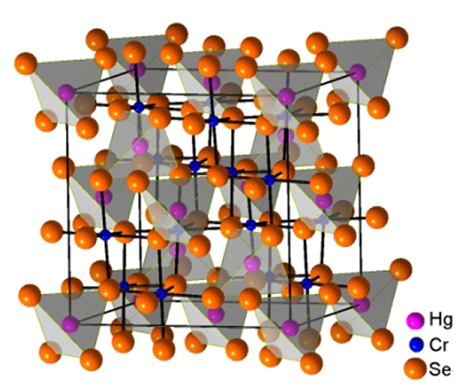
\includegraphics[height=0.7\linewidth]{spinel2.png}
\centering\captionof{figure}{The spinel crystal structure of HgCr$_2$Se$_4$ with Hg atoms in zinc-blende structure, each of them surrounded by Se tetrahedrons \cite{wang}. \label{spinel}}
\end{figure}

\begin{table}[h]
\centerline{\begin{tabular}{r|c|c|c|c|c|c|c}
  \hline \hline
   & \parbox{1.75cm}{Lattice parameter (\AA)} & \parbox{2.1cm}{ Resistivity, $\rho$, at 300 K ($\Omega\cdot$cm)} & \parbox{2.5cm}{Mobility, $\rho$, at 300 K (cm$^2\cdot$V$^{-1}\cdot$s$^{-1}$)} & \parbox{2.35cm}{\vspace{0.1cm} Magnetic moment at 4.2 K  ($\mu_B$/molecule)} & \parbox{1.8cm}{Curie temp., $T_c$ (K )}& \parbox{1.8cm}{Curie-Weiss, $\theta$ (K)} & \parbox{1.8cm}{Curie constant, $C_M$}\\
  \hline
  HgCr$_2$Se$_4$ & 10.753 & 0.7 & 30 & 5.64 & 106 & 200 & 3.79 \\
  \hline \hline
\end{tabular}}
\caption{Basic properties of HgCr$_2$Se$_4$ \cite{baltzer}\cite{lehmann}.} 
\end{table}

%%%%%%%%%%%%%%%%%%%%%%%%%%%%%%%%%%%%%%%%%%%%%%%%%%%%%%%%%%%
%%%%%%%%%%%%%%%%%%%%%%%%%%%%%%%%%%%%%%%%%%%%%%%%%%%%%%%%%%%

\section{Magnetic properties}

ferromagnets. figures are characteristic of compounds having a very low magnetic anisotropy. The magnetism in this material originate from the three 3d electrons on Cr3+ ions \cite{selmi}.

\noindent\begin{minipage}{0.39\linewidth}
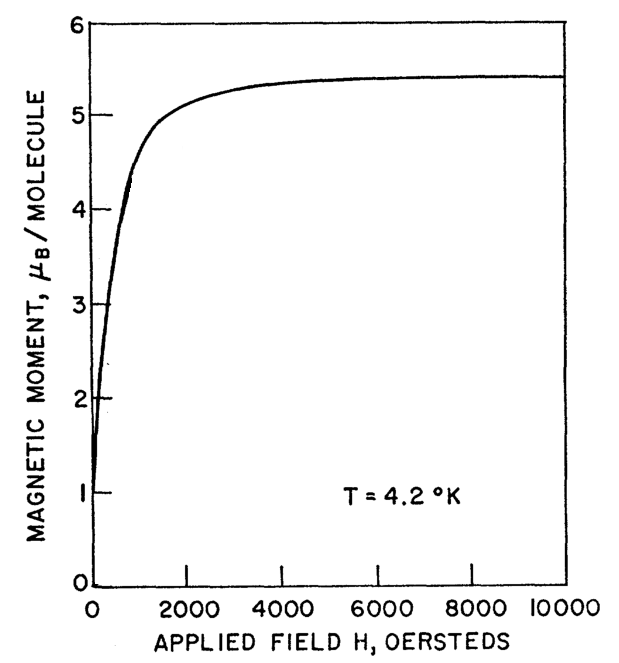
\includegraphics[width=1\linewidth]{momvsfield.png}
\centering\captionof{figure}{Magnetic moment as a function of applied field at 4.2 K \cite{baltzer}.\label{temp}}
\end{minipage}%
~ ~
\begin{minipage}{.59\linewidth}
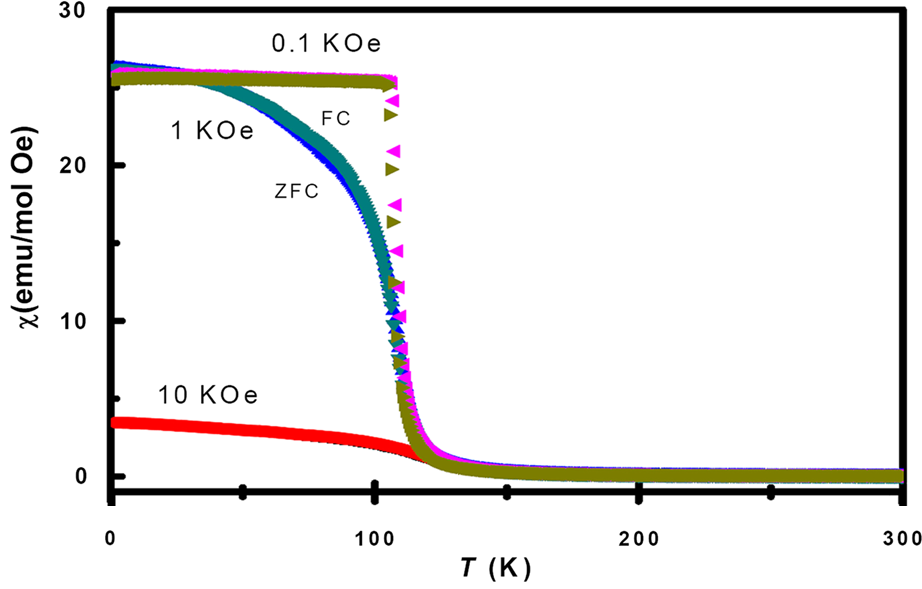
\includegraphics[width=1.1\linewidth]{suscvstemp.png}
\centering\captionof{figure}{Temperature dependence of the magnetic susceptibility for HgCr$_2$Se$_4$ \cite{wang}.\label{susc}}
%%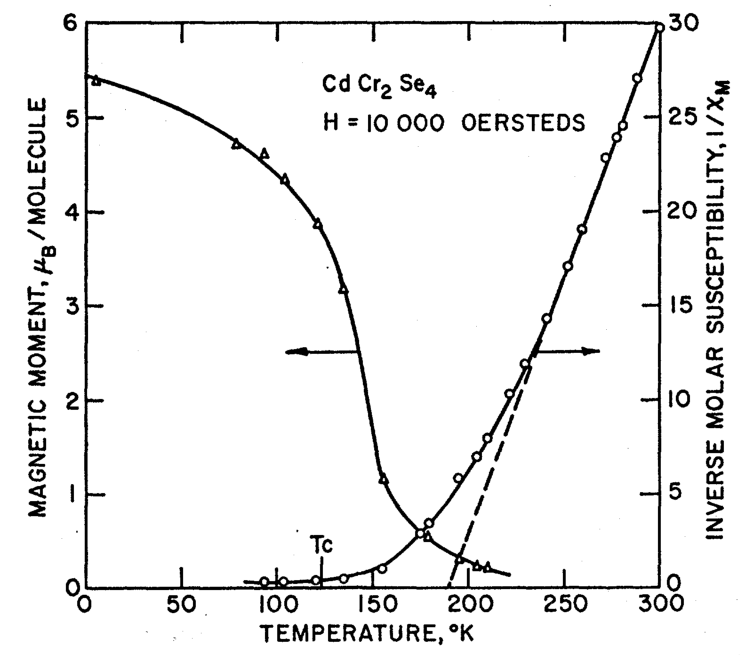
\includegraphics[height=0.95\linewidth]{momvstemp.png}
%\centering\captionof{figure}{Magnetic moment and inverse susceptibility as a function of temperature for CdCrgSe4 in an applied 6eld of 10000 Oe. HgCr$_2$Se$_4$ should have a similar behavior \cite{baltzer}.\label{field}}
\end{minipage}

%%%%%%%%%%%%%%%%%%%%%%%%%%%%%%%%%%%%%%%%%%%%%%%%%%%%%%%%%%%
%%%%%%%%%%%%%%%%%%%%%%%%%%%%%%%%%%%%%%%%%%%%%%%%%%%%%%%%%%%


\section{Transport properties: resistivity and hall effect}

good electrical insulators in addition to being ferromagnets, which is a rarity.
expected: DC-conductivity at low temperatures, negative magnetoresistance
 a dc voltage produced in the sample, and the other is a decrease in resistivity at ferromagnetic resonance at 77 K \cite{toda}. result from s-d exchange interactions.
 \cite{goldstein} details the effect of annealing at different pressures on the transport properties. p-type at room temperature, could be made n-type by annealing. exhibits a spontaneous Hall effect at 77 K. HgCr2Se4 has the smallest band gap among the chromium spinels. One paper \cite{selmi} reported different transport characteristics depending on the carrier density. Class I samples are those which fulfill the condition $n$ (4.2 K) \textgreater~$2\cdot10^{-3}$ cm$^{18}$. The main feature of such samples is that $n$ is roughly independent of $T$ below 200 K. To the contrary, for class II samples (n $\le$ $2\cdot10^{-3}$ cm$^{18}$), a sharp drop of $n$ at $T$ $\sim$ 120 K is observed, responsible for the peak of resistivity near T$_c$. In particular, the Hall mobility $\mu$ decreases monotonically near T$_c$ on all samples .

\begin{figure}[h]
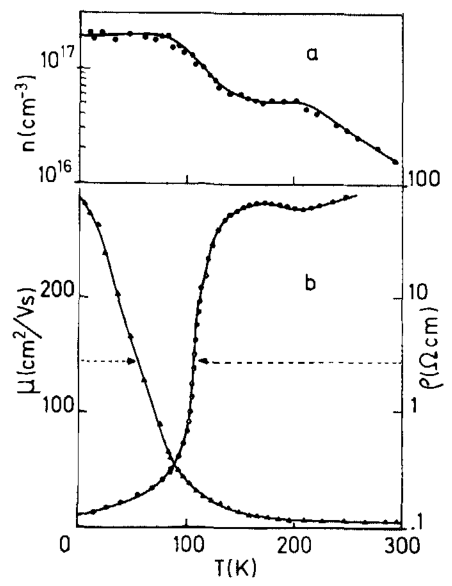
\includegraphics[height=0.7\linewidth]{mobvstemp.png}
\centering\captionof{figure}{Electron concentration, $n$ (a), resistivity, $\rho$, and mobility, $\mu$ (b) , vs.
temperature for the sample with smaller $n$ \cite{selmi}.  \label{mobility}}
\end{figure}

%%%%%%%%%%%%%%%%%%%%%%%%%%%%%%%%%%%%%%%%%%%%%%%%%%%%%%%%%%%
%%%%%%%%%%%%%%%%%%%%%%%%%%%%%%%%%%%%%%%%%%%%%%%%%%%%%%%%%%%

\section{Band structure}

%%%%%%%%%%%%%%%%%%%%%%%%%%%%%%%%%%%%%%%%%%%%%%%%%%%%%%%%%%%
%%%%%%%%%%%%%%%%%%%%%%%%%%%%%%%%%%%%%%%%%%%%%%%%%%%%%%%%%%%

\section{Specific heat}

\cite{wang}  weak AFM interaction, however it can compete with the FM interaction below low temperatures ($T < 3$ K)
and magnetic fields.

\noindent\begin{minipage}{0.54\linewidth}
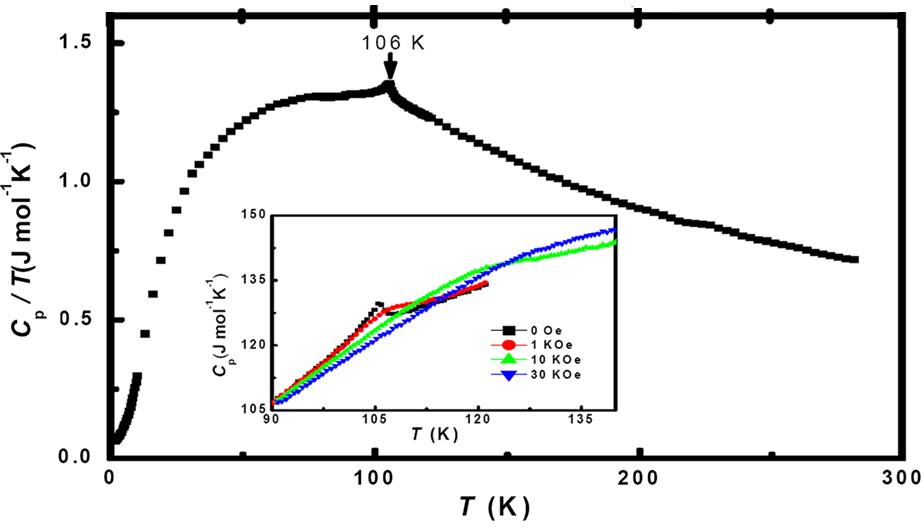
\includegraphics[width=1.07\linewidth]{heatvstemp.png}
\centering\captionof{figure}{The specific heat in the form $C_p$/$T$ vs. $T$. The inset shows the
vicinity of the magnetic transition at 106 K at different magnetic fields \cite{wang}. \label{heat}}
\end{minipage}%
~ ~ ~ ~
\begin{minipage}{.44\linewidth}
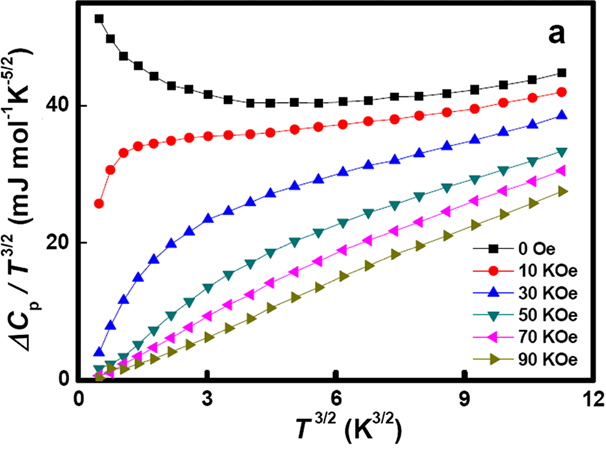
\includegraphics[width=1\linewidth]{dheatvstemp.png}
\centering\captionof{figure}{The divergence from $C_p=\alpha T+\delta T^{3/2}+\beta_DT^3$ at low temperatures indicating the competition between FM and AFM orders \cite{wang}.\label{dheat}}
\end{minipage}

%%%%%%%%%%%%%%%%%%%%%%%%%%%%%%%%%%%%%%%%%%%%%%%%%%%%%%%%%%%
%%%%%%%%%%%%%%%%%%%%%%%%%%%%%%%%%%%%%%%%%%%%%%%%%%%%%%%%%%%

\section{Comments on weyl semimetals}

Weyl nodes are stable as long as charge conservation and translational invariance is preserved. Disorder, in general, does not preserve the latter symmetry; however, if the disorder is smooth, many properties of the WSM that rely on the topological nature of the band structure should survive.

%%%%%%%%%%%%%%%%%%%%%%%%%%%%%%%%%%%%%%%%%%%%%%%%%%%%%%%%%%%
%%%%%%%%%%%%%%%%%%%%%%%%%%%%%%%%%%%%%%%%%%%%%%%%%%%%%%%%%%%
 
\section{Conclusions and future work}
\label{sec:conclusion}

%\begin{acknowledgments}
%\end{acknowledgments}
%%%%%%%%%%%%%%%%%%%%%%%%%%%%%%%%%%%%%%%%%%%%%%%%%%%%%%%%%%%
%%%%%%%%%%%%%%%%%%%%%%%%%%%%%%%%%%%%%%%%%%%%%%%%%%%%%%%%%%%



\bibliography{report}{}
\bibliographystyle{unsrt}

\end{document}             % End of document.

